\documentclass{subfiles}

\begin{document}
\subsubsection{Phasendiagramme}
	Wie schon erwähnt, können flüssige und gasförmige Phase eines Stoffes 		koexistieren. Im Gleichgewichtszustand bilanziert sich der Austausch von Molekülen an der Gas-Flüssigkeit-Grenzfläche also zu Null. In diesem Fall stellt sich ein bestimmter \textit{Dampfdruck} $p_s$ in der Dampfphase. Bei höheren Temperaturen überwinden mehr Moleküle die Oberflächenspannung der Flüssigkeitsphase, es wird also ein höherer Dampfdruck $p_s$ für Stabilität benötigt.\\
	
	\noindent Diagramm zeigt den qualitativen Verlauf der Dampfdruckkurve $p(T)$.
	
	\begin{figure}
		\centering
		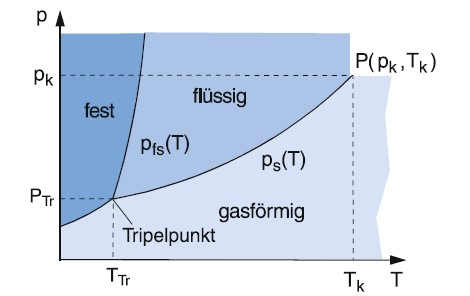
\includegraphics[width=7cm]{Bilddateien/Grundlagen/phasendiagramm.jpg}
		\caption{$p(T)$-\textit{Phasendiagramm}. Für einen Druck unterhalb der Dampfdruckkurve $p_s(T)$ liegt das System in gasförmiger Phase vor, oberhalb in flüssiger. Analog trennt die \textit{Schmelzkurve} $p_{ds}(T)$ die feste und flüssige Phase \cite[p.343]{demtroeder}}
		\label{fig:Dampfdruckkurve}
	\end{figure}
	Ebenso erwähnenswert sind zwei besondere Punkte im Diagramm:
	\begin{itemize}
		\item \textbf{Der Tripelpunkt}.	Im Tripelpunkt ist ein Gleichgewichtszustand möglich, wo alle drei Phasen des Stoffes koexistieren.
		\item \textbf{Der kritische Punkt}. Ab diesen Punkt $(T_{krit},p_{krit}$ lässt sich nicht mehr zwischen flüssiger und gasförmiger Phase unterscheiden; bei steigender Temperatur $T$ dehnt sich die Flüssigkeit aus, aber weil auch der Dampfdruck $p_s$ steigt, wird das Gas komprimiert. In kritischen Punkt haben beide Phasen letztlich dieselbe Dichte und sind identisch.
	\end{itemize}
	Im Gebiet oberhalb des kritischen Punkte im Phasendiagramm verortete Zustände heißen \textit{überkritschen Fluide} \cite[p.149]{heintze}.\\
	
\subsubsection{Bestimmung Kritischer Punkt}
	Der kritische Punkt ist nun auch über die Aufnahme mehrerer van-der-Waals-Isothermen zu sehen. Für jede Isotherme gibt die Höhe der Maxwell-Gerade den Dampfdruck an. Legt man eine Kurve über alle diese Geraden, ist die Fläche unter dieser Kurve gerade das Zustandsgebiet, wo Gasphase und die flüssige Phase koexistieren können. Deshalb wird das Gebiet auch \textit{Koexistenzgebiet} genannt (siehe auch ). 
	
	\begin{figure}
		\centering
		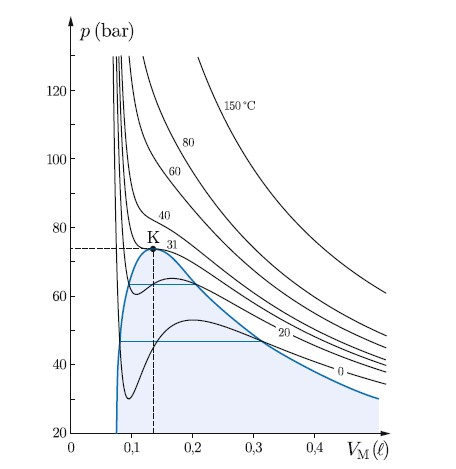
\includegraphics[width=5cm]{Bilddateien/Grundlagen/koexistenzgebiet.jpg}
		\caption{Koexistenzgebiet (blau) für reale Gase \cite[p.159]{heintze}}
	\end{figure}		
	Das Maximum der einhüllenden Kurve ist der kritische Punkt, wo der höchstmögliche Druck herrscht, bevor das Fluid überkritisch wird. Die Isotherme zu $T_{krit}$ hat in diesem Punkt also nicht nur eine Steigung von Null, sondern ist auch knickfrei. Aus \eqref{eq:VanDerWaals} lässt sich eine Funktion $p$ in Abhängigkeit von $T,V$ bestimmen. Für $p'(T_{krit},V_{krit})=0$ und $p''(T_{krit},V_{krit})=0$ lässt sich nun zeigen
	\begin{align*}
		V_{kr}&=3b\cdot n\\
		p_{kr}&=\frac{a}{27b^2}\\
		T_{kr}&=\frac{8}{27}\cdot\frac{a}{b}\cdot\frac{1}{R}
	\end{align*}
	Der kritische Punkt kann also grafisch bestimmt werden und anschließend zur direkten Bestimmung der Van der Waals-Koeffizienten genutzt werden \cite[p.158-159]{heintze}:
	\begin{align*}
		b&=\frac{27}{8}\cdot\frac{T_{kr}}{p_{kr}}\cdot R\\
		a&=27\cdot p_{kr}\cdot b^2
	\end{align*}
	Weiter ergibt sich die Stoffmenge als
	\begin{align*}
		n=\frac{3b}{V_{krit}}
	\end{align*}

\subsubsection{Die Clasius-Claperyon-Gleichung}
	Für \textbf{geschlossene} Systeme im Gleichgewicht muss überall auch die chemische Energie gleich sein (die als innere Energie neben Wärme und mechanische Arbeit im 1. Hauptsatz der Thermodynamik auftritt). Es lässt sich zeigen, dass in diesem Fall die Dampfdruckkurve $p_s$ Lösung der \textit{Clasius-Claperyon-Differentialgleichung} 
	\begin{align*}
		p_s'(T)=\frac{\Lambda}{T(V_{g}-V_{fl})}
	\end{align*}	 
	sein muss. Dabei sind $V_g$ und $V_{fl}$ je die Volumina der gasförmigen und flüssigen Phase und $\Lambda$ ist die Verdampfungswärme \cite[p.131-134]{nolting42}. Für ideale Gase ist $V_{fl}\ll V_{g}=\frac{n\cdot R\cdot T}{p}$ und $p_s$ ist in guter Näherung Lösung der vereinfachten Gleichung
	\begin{align*}
		p_s'(T)=\frac{p\cdot\Lambda}{n\cdot R\cdot T^2}.
	\end{align*}
	Die bis auf Startdaten eindeutige Lösung dieser Differentialgleichung ist aber bekannterweise von der Form
	\begin{align*}
		p_s=\fdef{A\cdot\exp(-\frac{\Lambda}{n\cdot R\cdot T})}{T\in\R_{>0}}.
	\end{align*}
	Auf diese Art lässt sich die Dampfdruckskurve und sogar Verdampfungswärme bestimmen.
    % -Vergleich p(V) Diagram für real, ideal (Maxwell-Geraden, Zweiphasengebiet, Darstellung kritischer Punkt in p(V), p(T)
    % -was ist ein überkritischer Fluid?
    % -Clasius-Claperyon-Gleichung
    % -Phasendiagramme + Phasengebieten (gas, flüssig, Koexistenzgebiet,
    %   kritscher Punkt

    % -Verdampfungskurve für Gleichgewicht flüssig-gas-Phase, Bedingung
    %   an Verdampfungsenthalpie, Dampfdruck!
  

    \subsubsection{Probestoff Schwefelhexafluorid}
        Im Versuch wird der Stoff Schwefelhexafluorid ($SF_6$) auf dessen thermodynamische Eigenschaften untersucht. Die räumliche Struktur ist in \ref{fig:SF6Struktur} dargestellt.
        \begin{figure}[H]
            \centering
            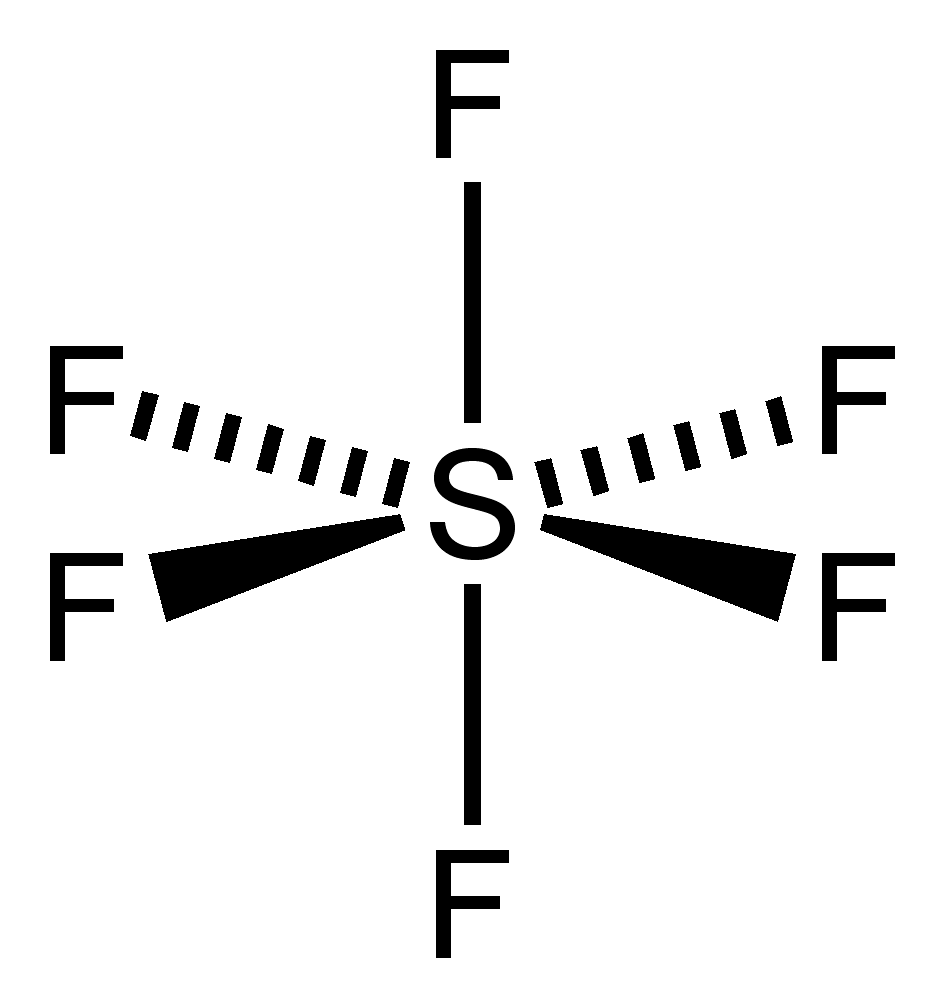
\includegraphics[width=4cm]{Bilddateien/Grundlagen/SF6.png}
            \caption{Räumliche Darstellung der Verbindung $SF_6$ \cite{SF6wiki}}
            \label{fig:SF6Struktur}
        \end{figure}

        \noindent Die Verbindung eignet sich, da sie ungiftig ist, nicht wärmeleitfähig und einen einfach im Labor erreichbaren kritischen Punkt hat, besonders gut für eine sichere, akkurate Messung. Konkret ist $T_{krit}=\SI{45.55}{\degree}$, $p_{krit}=\SI{37,6}{\bar}$ \cite{riessner}.
    % -speziell SF6: für Versuch relevante Literaturwerte und relevante %   Eigenschaften (Kritischer Punkt, Dampfdruck, etwas mit Enthalpie?
\end{document}